\chapter{CPU Virtualisation}

\section{The Abstraction: The Process}

\textbf{Process:} A running program.\\

\begin{tcolorbox}
    \textbf{Crux Of The Problem:} Although there are only a few physical CPUs
    available, how can the OS provide the illusion of nearly-endless supply of 
    said CPUs?\\
\end{tcolorbox}

The OS creates this illusion by \textbf{virtualizing} the CPU. By running
one process, then stopping it and running another, and so forth, the OS can
promote the illusion that many virtual CPUs exist when in fact there is only
one physical CPU (or a few). This technique is called \textbf{time-sharing}.\\

To do this, OS requires some low-level machinery and some
high-level intelligence. The low-level machinery is called \textbf{mechanisms}.
For example, stopping one program and starting another on a given CPU. On top
of these mechanisms, there is high-level intelligence call \textbf{policies}.
Policies are algorithms for making decisions within the OS.\\

Mechanisms: Provides answer to a \textit{how} question.

Policies: Provides answer to a \textit{which} question.

\section{Mechanism: Limited Direct Execution}

\begin{tcolorbox}
    \textbf{The Crux:} How to efficiently virtualize the CPU with control?
\end{tcolorbox}

The OS must virtualize the CPU in an efficient manner while retaining control
over the system. To do so, both hardware and operating-system support will be
required. The OS will often use a judicious bit of hardware support in order to
accomplish its work effectively.

\subsection{Basic Technique: Limited Direct Execution}

The \textit{direct execution} part of the idea: just run the program directly
on the CPU. Thus, when the OS wishes to start a program, it creates a process
entry for it in a process list, allocates some memory for it, loads the program
code into memory, locates its entry point (main()), jumps to it, and starts
running the user's code.\\

This approach gives rise to a few problems:

\begin{itemize}
    \item How to make sure that the program does not do anything that we don't
        want it to do while still maintaining efficiency?
    \item How do we stop a process and switch to another process, i.e. how
        to implement \textbf{time sharing} we require to virtualize the CPU?
\end{itemize}

\subsubsection{Problem \#1: Restricted Operations}

What if the process wishes to perform some kind of restricted operation, such
as issuing an I/O request to a disk, or gaining access to more system resources
such as CPU or memory?\\

\begin{tcolorbox}
    \textbf{The Crux: How to perform restricted operations}

    A process must be able
    to perform I/O and some other restricted operations, but without giving the
    process complete control over the system.\\
\end{tcolorbox}

Two different modes:

\begin{itemize}
    \item \textbf{User Mode:} Code that runs in user mode is restricted in what
        it can do. For example, when running in user mode, a process can't
        issue I/O requests; doing so would result in the processor raising an
        exception.
    \item \textbf{Kernel Mode:} Mode the operating system (or kernel) runs in.
        In this mode, code that runs can do whatever it likes, including
        privileged operations such as issuing I/O requests and executing
        restricted instructions.
\end{itemize}

All modern hardware provides the ability for user programs to perform a 
\textbf{system call}. System calls allow the kernel to carefully expose
certain key pieces of functionality to user programs such as accessing the file
system, creating and destroying the processes, communicating with other
processes, and allocating more memory.

\paragraph{System calls}

To execute a system call, a program must execute a special \textbf{trap}
instruction. This instruction jumps into the kernel and raises privilege level
to kernel mode; once in the kernel, the system can now perform the restricted 
operations needed and thus the required work for the calling process. When 
finished, the OS calls a special \textbf{return-from-trap} instruction, which
returns into the calling user program while simultaneously reducing the 
privilege level back to user mode.\\

When executing a trap, the caller's registers must be saved in order to 
return correctly when the OS issues the return-from-trap instruction.\\

On x86, the processor will push the program counter, flags and a few other
registers onto a per-process \textbf{kernel stack}; return-from-trap
will pop these values from the stack and resume execution.

\paragraph{How does the trap know which code to run inside the OS?}

Clearly, the calling process can't specify and address to jump to; doing so 
would allow programs to jump anywhere into the kernel which is not secure. The
kernel must control what code executes upon a trap.\\

The kernel does so by setting up a \textbf{trap table} at boot time. When the
machine boots up, it does so in kernel mode. One of the first things the OS
does is to tell the hardware what code to run when certain exceptional events
occur. The OS informs the hardware of these locations of these
\textbf{trap handlers}, usually with some kind of special instruction. Once
the hardware is informed, it remembers the location of these handlers until
the machine is rebooted, and thus hardware knows what to do when system calls
and other exceptional events take place.\\

To perform the exact system call, a \textbf{system-call number} is usually 
assigned to each system call. The user code has to place the desired system-call
number in a register or at a specific location in the stack; the OS, when
handling the system call inside the trap handler, examines the number,
ensures it is valid, and, if it is, executes the corresponding code. This
level of indirection serves as a form of \textbf{protection}; user code cannot
specify an exact address to jump to, but rather must request a particular 
service via a number.\\

Telling the hardware where the trap tables are is a \textbf{privileged} 
operating, otherwise you could make your own trap tables and compromise the
system.\\

How all this works:

\begin{enumerate}
    \item At boot time, the kernel initializes the trap table, and the CPU
        remembers its location for subsequent use. The kernel does so via
        a privileged instruction.
    \item The kernel sets up a few things (allocating memory, etc.) before
        using a return-from-trap instruction to start the execution of the 
        process. When the process wishes to issue a system call, it traps back
        into the OS, which handles it and once again returns control via a 
        return-from-trap to the process. The process completes its work and 
        returns from main().
\end{enumerate}

\subsubsection{Problem \#2: Switching Between Processes}

When a process is running on the CPU, this by definition means the OS is
\textit{not} running. If OS isn't running how can
it change a process? (it cant).\\

\begin{tcolorbox}
    \textbf{The Crux: How to regain control of the CPU?}

    How can the operating system \textbf{regain control} of the CPU so that it can
    switch between processes?
\end{tcolorbox}

\paragraph{Cooperative Approach: Wait for system calls}

In this approach, the OS regains control of the CPU by waiting for a 
system call or an illegal operation of some kind to take place, as
control is passed to the OS during these exceptions.

\paragraph{Non-Cooperative Approach: The OS takes control}

If we get stuck in an infinite loop in the cooperative approach, the only way
out is to reboot the machine.\\

\begin{tcolorbox}
    \textbf{The Crux: How to gain control without cooperation} 

    How can the OS gain control of the CPU even if processes are not being
    cooperative? What can the OS do to ensure a rogue process does not take over
    the machine?\\
\end{tcolorbox}

\textbf{Timer interrupt:} A timer device is programmed to raise an interrupt
after a fixed delay; when the interrupt is raised, the currently running
process is halted, and a pre-configured \textbf{interrupt handler} in the OS
runs. Now the OS has regained control of the CPU, and thus can stop the 
current process and start a different one.\\

At boot time, the OS starts the interrupt timer. This is a privileged
operation.

\paragraph{Saving and Restoring Context}

The OS has regained control now. It can decide to switch or not. This decision
is made by the \textbf{scheduler}.\\

If the decision is to switch, the OS executes a \textbf{context switch}. A
context switch saves register values of the currently-executing process and
restores register values for the soon-to-be-executing process. After this, 
the OS executes a return-from-trap instruction and executes the new process.\\

By switching stacks pointers (stack pointer is a register),
the kernel enters call to the switch code in the 
context of one process (the interrupted one) and returns in the context of
another (the soon-to-be-executing one). By switching stack is actually how the
process is switched.\\

There are two types of register saves/restores that happen here:

\begin{itemize}
    \item When the timer interrupt occurs. The \textit{user registers} of the
        running process are implicitly saved by the \textit{hardware}, using
        the kernel stack of the process.
    \item When OS performs the context switch. The \textit{kernel registers} 
        are explicitly saved by the \textit{software} (i.e. the OS), but this
        time into memory in the process structure of the process.
\end{itemize}

More info on the last two points \href{https://cs.stackexchange.com/questions/96550/whats-the-difference-between-user-registers-and-kernel-registers}{here}

\section{Scheduling}

In this section we will understand \textbf{policies} that OS scheduling
employs.\\

\begin{tcolorbox}
    \textbf{The Crux: How To Develop Scheduling Policy}\\

    How should we develop a basic framework for thinking about scheduling
    policies? What are the key assumptions? What metrics are important? What
    basic approaches have been used in earliest of computer systems?
\end{tcolorbox}

We will make some assumptions and continue to relax them to get to an optimal
policy. Assumptions:

\begin{enumerate}
    \item Each job runs for the same amount of time.
    \item All jobs arrive at the same time.
    \item Once started, each job runs to completion
    \item All jobs only use the CPU (i.e., they perform no I/O)
    \item The run-time of each job is known
\end{enumerate}

For now, we will use a single metric to determine optimal policy:
\textbf{turnaround time}.

$$
T_{turnaround} = T_{completion} - T_{arrival}
$$

\subsection{First In, First Out (FIFO)}

\begin{figure}[h!]
    \begin{center}
        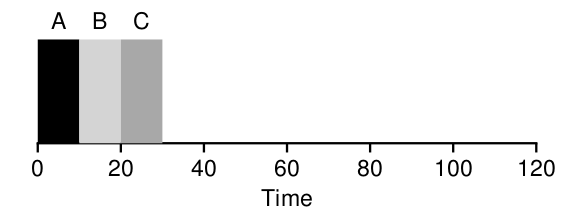
\includegraphics[width=5cm]{img/71.png}
        \caption{FIFO Simple Example}
    \end{center}
\end{figure}

For our current assumptions, this is optimal. But if we relax the assumption
that job running time are same, we can get bad turnaround time:

\begin{figure}[h!]
    \begin{center}
        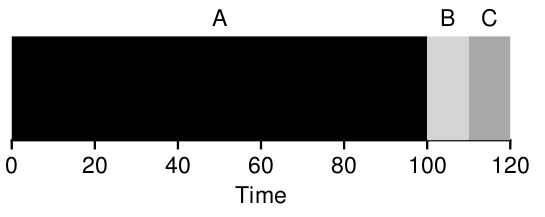
\includegraphics[width=5cm]{img/72.png}
        \caption{Why FIFO is Not that Great}
    \end{center}
\end{figure}

\subsection{Shortest Job First (SJF)}

\begin{figure}[h!]
    \begin{center}
        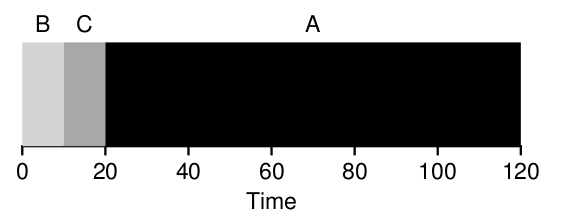
\includegraphics[width=5cm]{img/73.png}
        \caption{SJF Simple Example}
    \end{center}
\end{figure}

It can be proven that under these assumptions, SJF will give the best
turnaround time.\\

Now, lets relax the assumption that all jobs arrive  at the same time. Now,
we can build a worst case for SJF:

\begin{figure}[h!]
    \begin{center}
        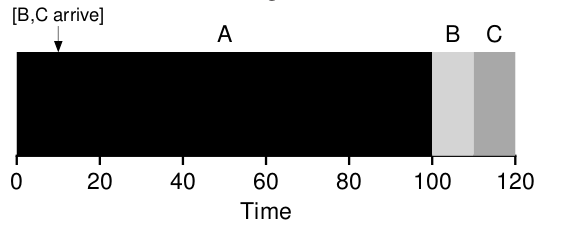
\includegraphics[width=5cm]{img/74}
        \caption{SJF With Late Arrivals from B and C}
        \label{74}
    \end{center}
\end{figure}

\subsection{Shortest Time-To-Completion First (STCF)}

To address this concern, we need to relax assumption 3 (jobs started, must run
to completion). SJF by our definition was a \textbf{non-preemptive} scheduler,
and thus suffered from the problems in figure \ref{74}.\\

To improve upon that, we add preemption to SJF, known as STCF. Any time
a new job enters the system, the STCF scheduler determines which of the
remaining jobs has least time left, and schedules that. It can be proven
that under the current assumptions, this is the best scheduler
(w.r.t turnaround time)

\begin{figure}[h!]
    \begin{center}
        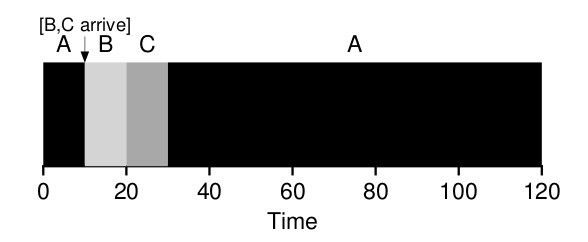
\includegraphics[width=5cm]{img/75}
        \caption{STCF Simple Example}
    \end{center}
\end{figure}

\textbf{New Metric: Response Time}: If our only metric was turnaround time and
we knew job runtime, STCF would be a great policy. But introduction of
time-sharing machines, required interactive performance from system as well.
Thus a new metric was needed: \textbf{response time}

$$
T_{response} = T_{firstrun} - T_{arrival}
$$

\subsection{Round Robin}

To improve upon response time, we introduce \textbf{Round-Robin (RR)}
scheduling. Basic idea: Instead of running a job to completion, RR runs a job
for a \textbf{time slice} (or \textbf{scheduling quantum}) and then switches
to the next job in the run queue.\\

The length of time-slice is obviously a multiple of timer-interupt.\\

\begin{figure}[h!]
    \begin{center}
        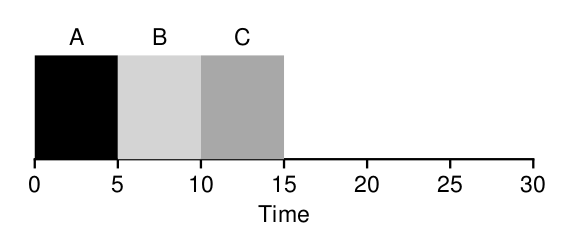
\includegraphics[width=4cm]{img/76}
        \caption{SJF (Bad response time)}
    \end{center}
\end{figure}

\begin{figure}[h!]
    \begin{center}
        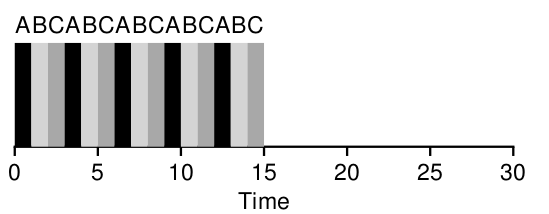
\includegraphics[width=4cm]{img/77}
        \caption{RR (Good response time)}
    \end{center}
\end{figure}

The length of time slice is critical for RR. The shorter it is, the better
performance of RR under response-time metric. However, too small time-slice can
result in time taken to context switch to dominate overall performance. Thus,
time slices should be made long enough to  \textbf{amortize} the cost of
switching without making it so long that system is no longer responsive.\\

RR is one of the \textit{worst} policies for turnaround time because it extends
the program to as long as possible.

\subsubsection{Incorporating I/O}

We now relax assumption that there is no I/O. When a job initiates an I/O
request, because the currently-running job won't be using the CPU during the
I/O; it is \textbf{blocked} waiting for the I/O completion. The CPU is idle
during the time of the I/O.\\

The scheduler incorporates I/O by treating each CPU burst as a job. the
scheduler makes sure processes that are "interactive" get run frequently. While
those interactive jobs are performing I/O, other CPU-intensive jobs run, thus
better utilizing the processor.

\subsection{The Multi-Level Feedback Queue}

In this subsection, we remove the assumption that we know job time and 
we will describe the most well-known approach to
scheduling, \textbf{MLFQ}. \\

\begin{tcolorbox}
    \textbf{The Crux: How To Schedule Without Perfect Knowledge?}\\

    How can we design a scheduler that both minimizes response time for
    interactive jobs while also minimizing turnaround time without a
    \textit{prior} knowledge of job length?\\
\end{tcolorbox}

MLFQ has a number of distinct \textbf{queues}, each assigned a different 
\textbf{priority level}. MLFQ uses priorities to decide which job should run
at a given time. Basic rules for MLFQ:

\begin{enumerate}
    \item If Priority(A) $>$ Priority(B), A runs (B doesn't)
    \item If Priority(A) = Priority(B), A \& B run in RR.
\end{enumerate}

Rather than giving a fixed priority to each job, MLFQ \textit{varies} the
priority of a job based on its \textit{observed behavior}.\\

If a job repeatedly relinquishes the CPU while
waiting for input from the keyboard, 
MLFQ will keep its priority high, as this is how an interactive process might
behave. If a job uses the CPU intensively for long periods of time, MLFQ will
reduce its priority. In this way, MLFQ will try to \textit{learn} about 
processes as they run, and thus use the \textit{history} of the job to
predict its \textit{future} behavior.

\begin{figure}[h!]
    \begin{center}
        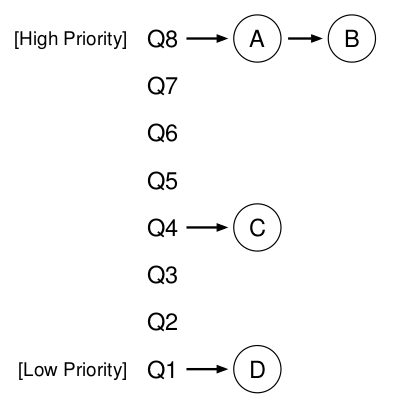
\includegraphics[width=5cm]{img/81.png}
        \caption{MLFQ Example}
    \end{center}
\end{figure}

\subsubsection{Attempt \#1: How to Change Priority}

Keep in mind: Our workload contains a mix of interactive jobs that are short
running (and may frequently relinquish the CPU), and some longer running
"CPU-bound" jobs that need a lot of CPU time but where the response time
isn't important. Here is the first attempt at an algorithm:

\begin{enumerate}
        \setcounter{enumi}{2}
    \item When a job enters the system, it is placed at highest
        priority (the topmost queue)
    \item 
        \begin{itemize}
            \item If a job uses up an entire time slice while running, 
                its priority is \textit{reduced}.
            \item If a job gives up the CPU before the time slice is up,
                it status at the \textit{same} priority level.
        \end{itemize}
\end{enumerate}

\subsection{Problems with current MLFQ}

There is a problem of \textbf{starvation:} if there are "too many" interactive
jobs in the system, they will combine to consume \textit{all} CPU time, and
thus long-running jobs will \textit{never} receive any CPU time.\\

Another problem is that the scheduler can be \textbf{gamed}. Gaming a scheduler
refers to the idea to tricking the scheduler in giving more time than the job's
share. Before the time-slice is over, the job could issue and I/O and remain
at the same priority. Doing so, allows the program to gain a higher percentage
of CPU time.

\subsection{Attempt \#2: The Priority Boost}

We add a new rule to handle the flaws. 

\begin{enumerate}
        \setcounter{enumi}{4}
    \item After some time period $S$, move all the jobs in the system to the
        topmost queue.
\end{enumerate}

This solves the problem of starvation. $S$ has to be set properly.

\subsection{Attempt \#3: Better Accounting}

We rewrite Rule 4 to make it anti-gaming.

\begin{enumerate}
        \setcounter{enumi}{3}
    \item Once a job uses its time allotment at a given level (regardless of
        how many times it has given up the CPU), its priority is reduced.
\end{enumerate}

\begin{tcolorbox}
    \textbf{MLFQ: Summary}
    \begin{enumerate}
        \item If Priority(A) $>$ Priority(B), A runs (B doesn't)
        \item If Priority(A) = Priority(b), A \& B run in round-robin fashion
            using the time slice of the given queue.
        \item When a job enters the system, it is placed at the highest
            priority.
        \item Once a job uses up its time allotment at a given level, its
            priority is reduced.
        \item After some period $S$, move all jobs to the topmost queue.
    \end{enumerate}
\end{tcolorbox}
